%!TEX root = Main.tex

\section{Simulation} \label{sec:simulation}

In the first case we analyze the network with two types of nodes.
Figure \ref{fig: nodes locations} shows the locations of 50 nodes, among which 4 are from type I and the rest 46 are from type II.
The first type of nodes (type I) are equispaced points on $x=0.5$ and $0.8\leq y\leq 5.2$.
The second type of nodes (type II) are generated uniformly in $[0,1]\times[0,6]$. 
\\
\begin{figure}[htbp]
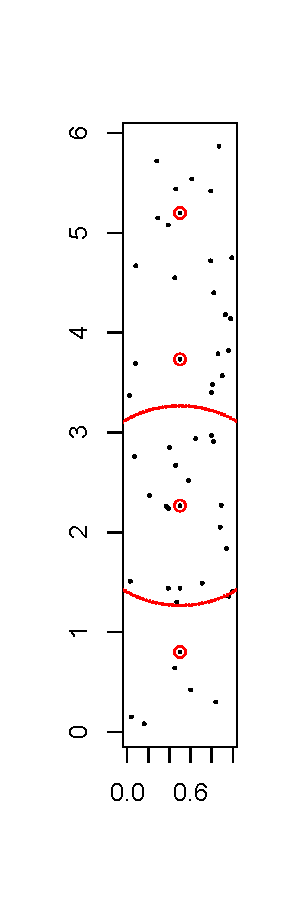
\includegraphics[width=.2\linewidth]{../simulation/plots/nodes_1_108}
\caption{Case 1. Locations of nodes. Each black dot represents a node, the four type I nodes are marked as red. The dotted circle explains the reachable area of the second type I node. }
\label{fig: nodes locations}
\end{figure}

\noindent
The network is developed during time period $[0,50]$.
Two nodes are connected if the distance between them is less than $1$.
The connecting time between two type II nodes is generated from uniform distribution $U(0,40)$.
For the pair of nodes with one from type I and the other from type II, the connecting time is distributed as $N(5+\tau,1)$, where $\tau$ is the time delay caused by the type I node and is generated randomly from $U(0,30)$.

\noindent
Figure \ref{fig: original curves} shows the empirical distribution function of the connecting time of each node.
Figure \ref{fig: aligned curves} shows clustering result. All nodes except one type II node are clustered correctly.


% Due to the uncertainty caused by initialization, five independent initializations are used for each trial, and only the one with the largest distance between estimated mean curves is kept.
\noindent
The k-means++ initialization method is performed. 
For each trial, three independent initializations are conducted, and only the one leading to the largest 
between-cluster distance
is kept, where the between-cluster distance is defined as the minimum pairwise distance between estimated mean  functions.
The clustering result is measured using adjusted rand index (ARI), which is also used in \citet{Matias2018}.
The algorithm is tested in 1000 synthetic networks. 
The ARI is compared between trials with or without good initialization, and the result is shown in Figure \ref{fig: ARI, case1}.


\begin{figure}
\begin{subfigure}{.45\textwidth}
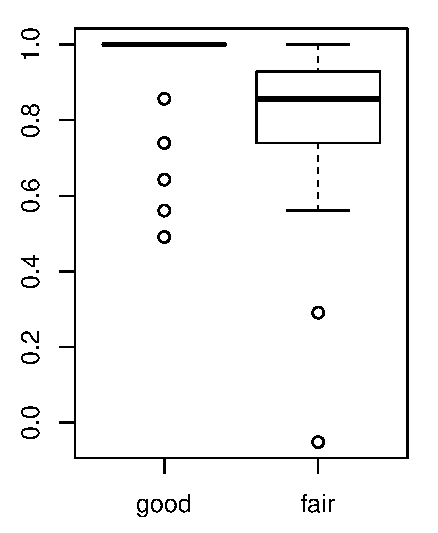
\includegraphics[width=\linewidth]{../simulation/plots/ARI_vs_init_case1.pdf}
\caption{}
\label{fig: ARI boxplot, case 1}
\end{subfigure}
\begin{subfigure}{.45\textwidth}
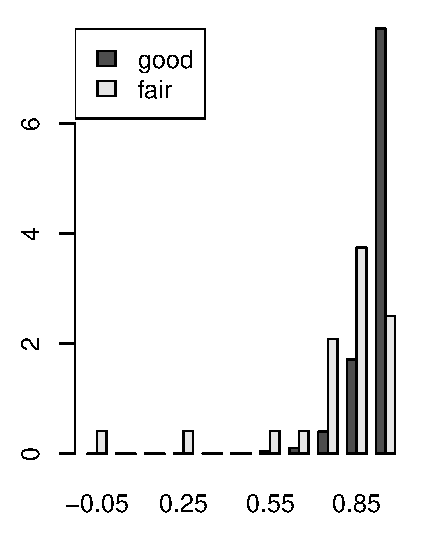
\includegraphics[width=\linewidth]{../simulation/plots/ARI_hist_case1}
\caption{}
\label{fig: ARI hist, case 1}
\end{subfigure}
\caption{Case 1. ARI for trials with good initialization (``good'') and trials without good initialization (``fair'').
$n_{good}=976, n_{fair}=24.$
}
\label{fig: ARI, case1}
\end{figure}




The second case is with three clusters.
The locations of nodes are displayed in Figure \ref{fig: nodes locations, case 2}.
The connecting radius for type I node is set as $2$, and that for other nodes is set as $1$. 
For a pair of type III nodes, the connecting time is generated from uniform distribution $U(0,30)$.
For the pair of nodes with one from type II and the other from type III, 
the connecting time is distributed as $N(5+\tau,1)$, where $\tau$ is the time delay caused by the type II node and is generated randomly from $U(0,10)$.
For the pair of nodes with one from type I and the other from type II, the connecting time is distributed as $U(\tau,\tau+6)$, where $\tau$ is the time delay caused by the type II node and is generated randomly from $U(40,42)$.

\begin{figure}[]
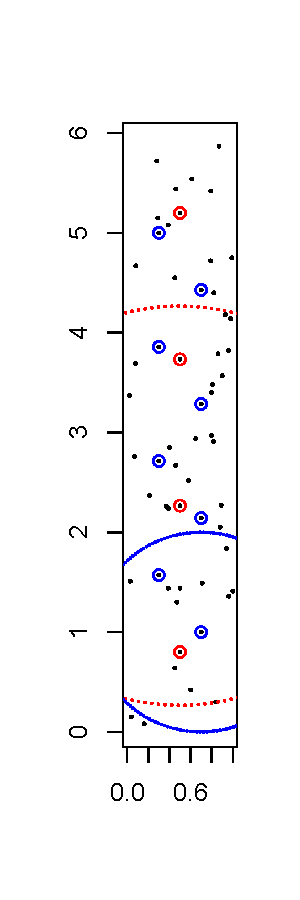
\includegraphics[width=.2\linewidth]{../simulation/plots/nodes_2_108}
\caption{Case 2. Locations of nodes. Each black dot represents a node, the four type I nodes are marked as red, and eight type II nodes are marked as blue. The dotted red and blue circles explain the reachable area of the type I node and type II node, respectively. }
\label{fig: nodes locations, case 2}
\end{figure}

\noindent
Figure \ref{fig: original curves, case 2} shows the empirical distribution function of the connecting time of each node. Due to the time delay of type I node, the distribution function of type II nodes are not identically distributed anymore.
Figure \ref{fig: aligned curves, case 2} shows clustering result. All nodes except four type III node are clustered correctly.
\\
1000 independent trials are recorded. 
The k-means++ initialization is applied for each trial.
The ARI is displayed in Figure \ref{fig: ARI, case2}.


\begin{figure}
\begin{subfigure}{.45\textwidth}
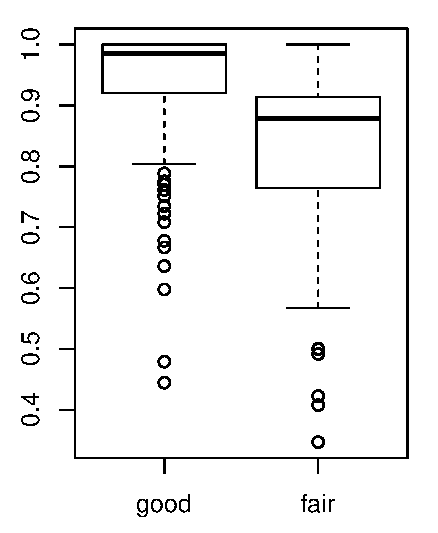
\includegraphics[width=\linewidth]{../simulation/plots/ARI_vs_init_case2}
\caption{}
\label{fig: ARI boxplot, case 2}
\end{subfigure}
\begin{subfigure}{.45\textwidth}
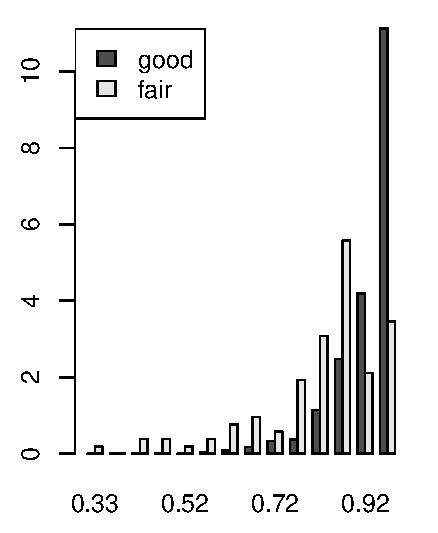
\includegraphics[width=\linewidth]{../simulation/plots/ARI_hist_case2}
\caption{}
\label{fig: ARI hist, case 2}
\end{subfigure}
\caption{Case 2. ARI for trials with good initialization (``good'') and trials without good initialization (``fair'').
$n_{good}=896, n_{fair}=104.$
}
\label{fig: ARI, case2}
\end{figure}


The third case has almost the same set up as Case 2, except that 
the time delays of the type II nodes are generated from $U(0,30)$ (it was $U(0,10)$ in the second case).
One trial is displayed in Figure 
to show the empirical distribution functions before and after cluster (and alignment).

\begin{figure}
\begin{subfigure}{.45\textwidth}
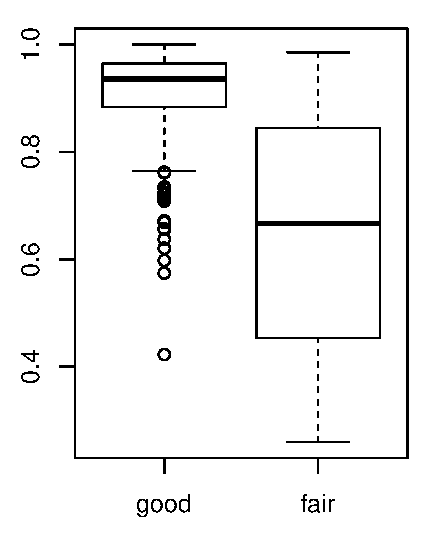
\includegraphics[width=\linewidth]{../simulation/plots/ARI_vs_init_case3}
\caption{}
\label{fig: ARI boxplot, case 3}
\end{subfigure}
\begin{subfigure}{.45\textwidth}
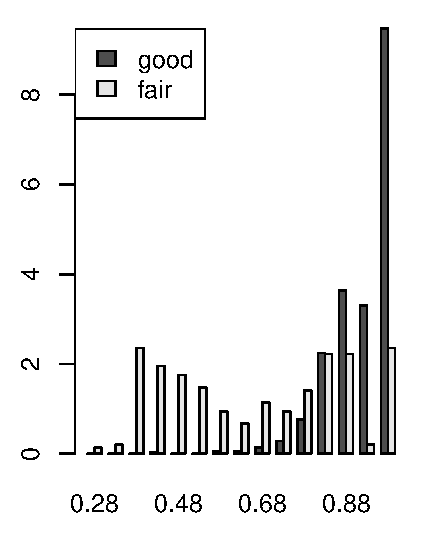
\includegraphics[width=\linewidth]{../simulation/plots/ARI_hist_case3}
\caption{}
\label{fig: ARI hist, case 3}
\end{subfigure}
\caption{Case 3. ARI for trials with good initialization (``good'') and trials without good initialization (``fair''). $n_{good}=703, n_{fair}=297.$
}
\label{fig: ARI, case3}
\end{figure}

\noindent
1000 independent trials are recorded. 
The k-means++ initialization is applied for each trial.
The ARI is displayed in Figure \ref{fig: ARI, case3}.


\begin{figure}[H]
\begin{subfigure}{.45\textwidth}
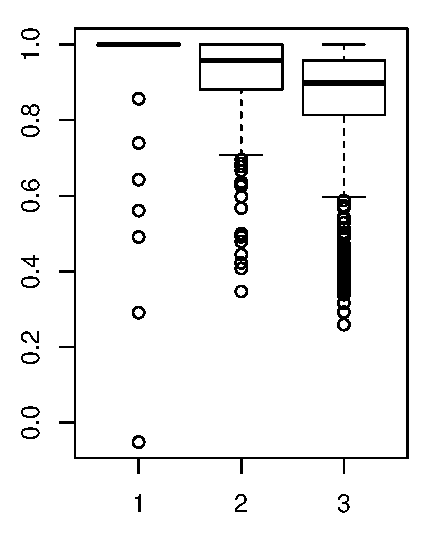
\includegraphics[width=\linewidth]{../simulation/plots/ARIall_123_boxplot}
\caption{}
\label{fig: ARI boxplot cmpr, all clus}
\end{subfigure}
\begin{subfigure}{.45\textwidth}
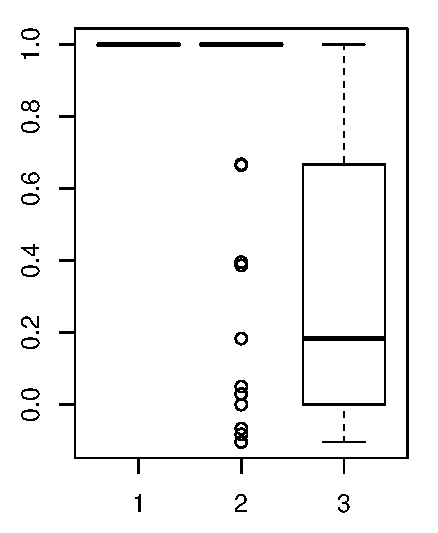
\includegraphics[width=\linewidth]{../simulation/plots/ARI_4or12_123_boxplot}
\caption{}
\label{fig: ARI boxplot cmpr, impt clus only}
\end{subfigure}
\caption{Comparison of three cases. (a): ARI over all nodes. (b): ARI over nodes in important clusters (type I nodes for case 1, type I\&II nodes for case 2 and case 3)
}
\label{fig: ARI boxplot cmpr}
\end{figure}

\noindent
The comparison between three cases is performed in Figure \ref{fig: ARI boxplot cmpr}.


[Need to add plots for estimated mean intensities.]

% To show the development of the network, we plot snapshots in Fig.\ref{Fig: development of network} of the network $\mathbf{G}_1$  at time points $t=0.01, 0.1, 1, 10, 100$.
% \begin{figure}
% \centering
% 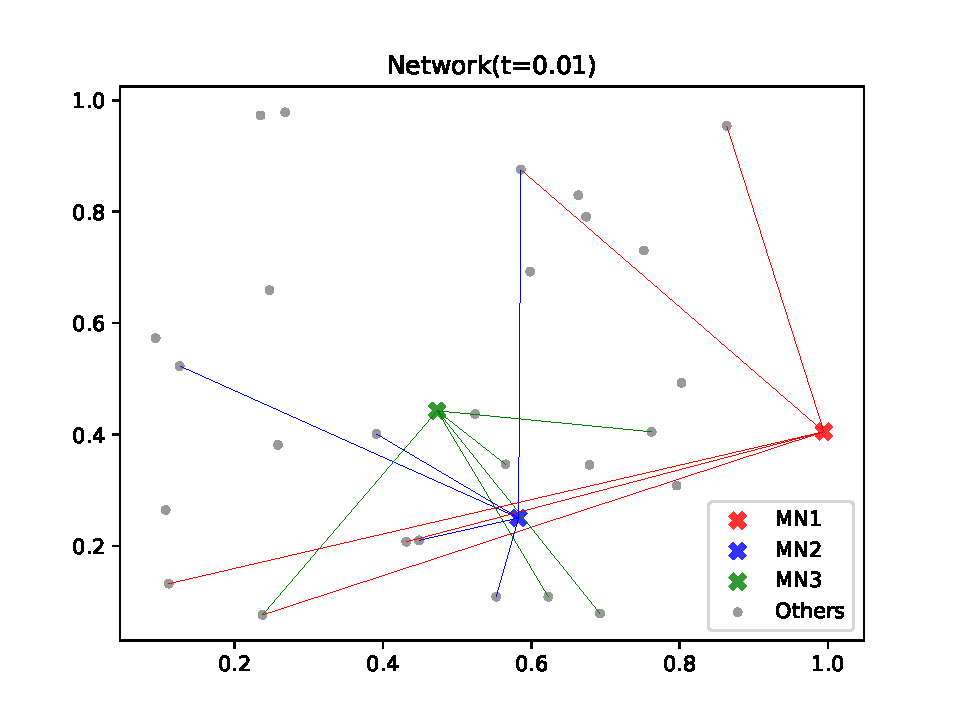
\includegraphics[width = 0.3\textwidth]{Graphs/t_001.pdf}
% 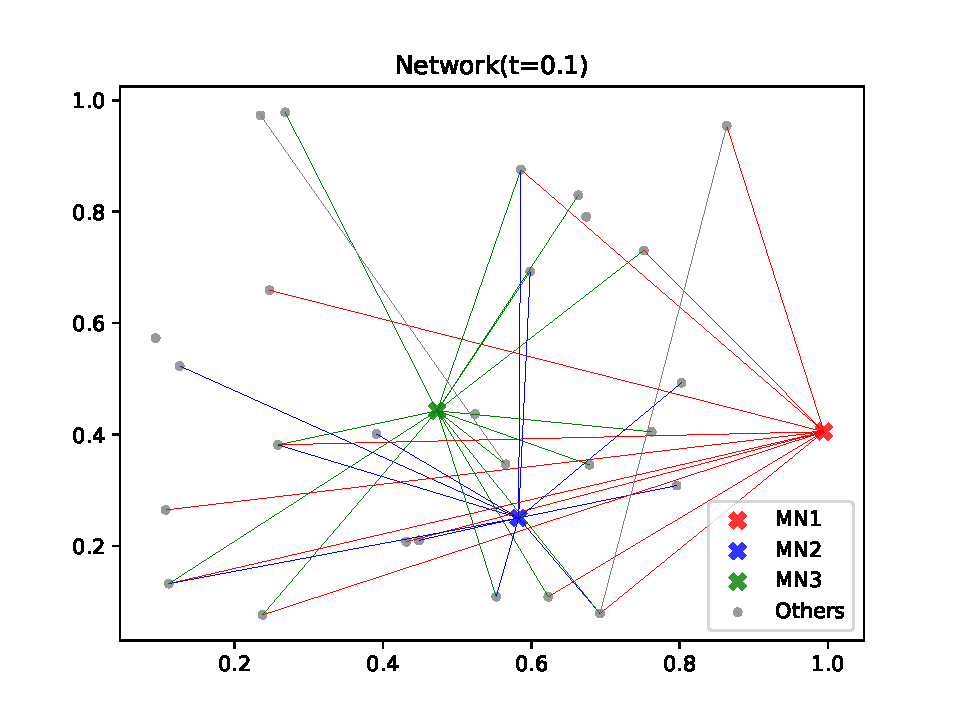
\includegraphics[width = 0.3\textwidth]{Graphs/t_01.pdf}
% 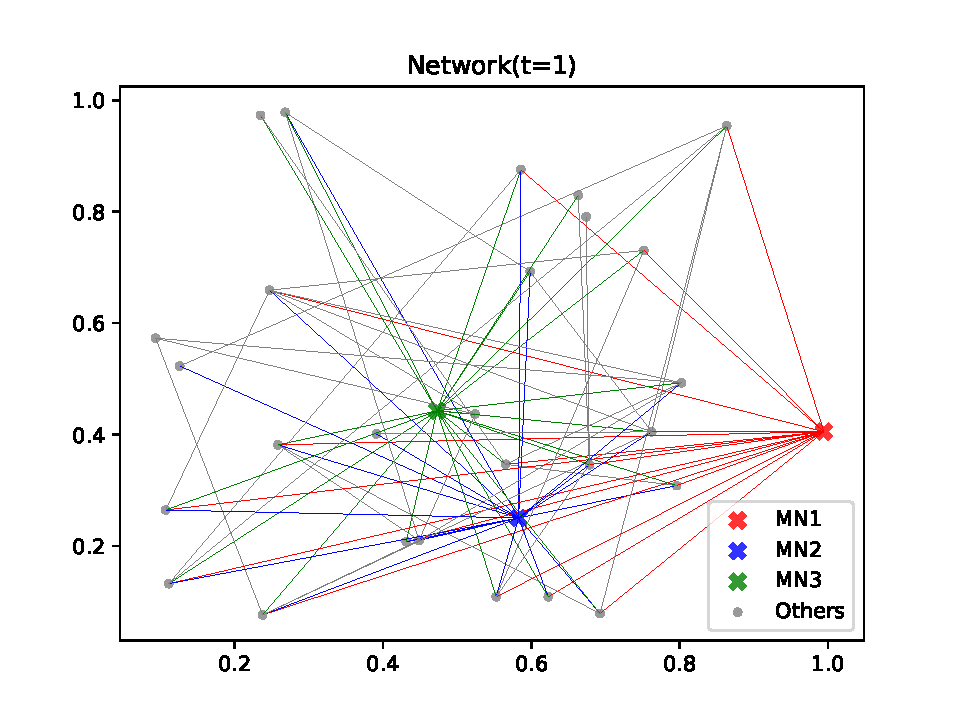
\includegraphics[width = 0.3\textwidth]{Graphs/t_1.pdf}\\
% 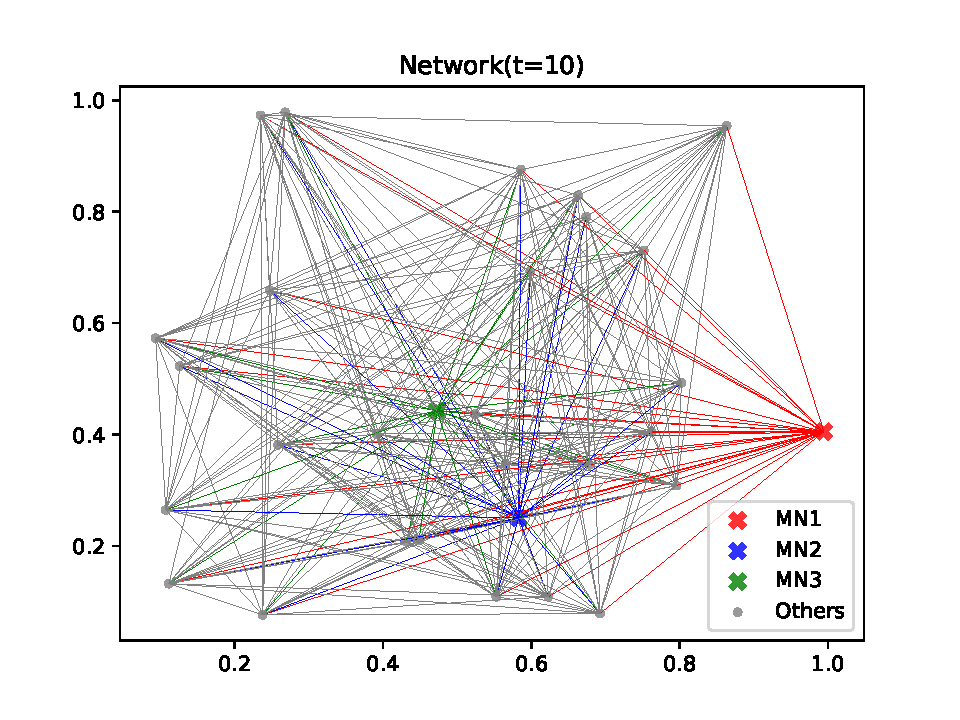
\includegraphics[width = 0.3\textwidth]{Graphs/t_10.pdf}
% 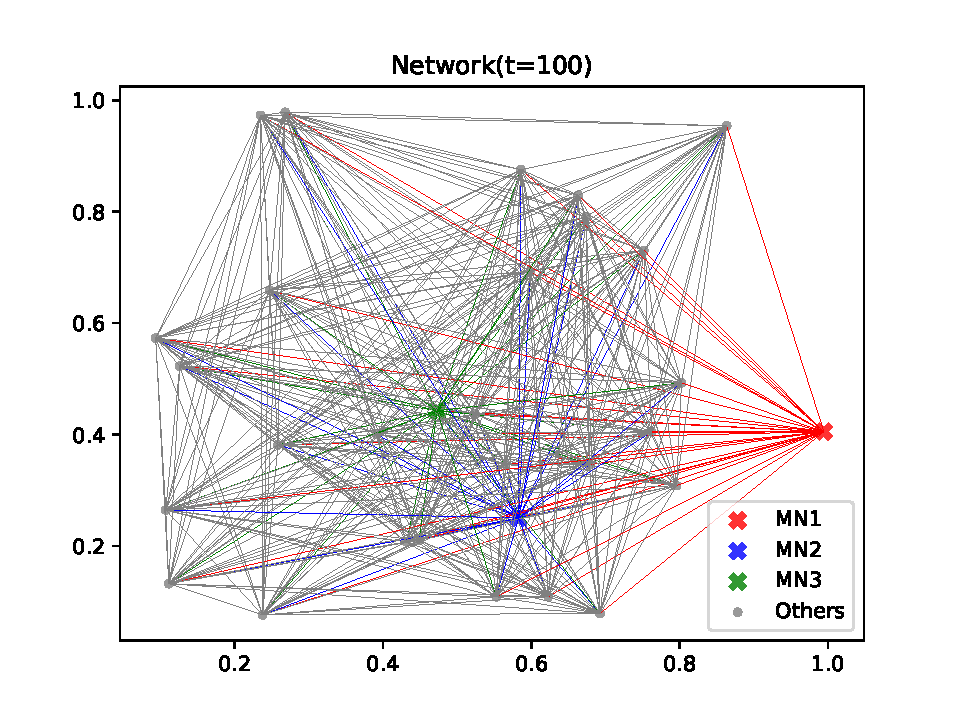
\includegraphics[width = 0.3\textwidth]{Graphs/t_100.pdf}
% \caption{Development of the network with two cell types. The node $n_1$ is represented by ``MN1'' in red. The node $n_2$ is represented by ``MN2'' in blue. The node $n_3$ is represented by ``MN3'' in green. Other nodes are represented by ``Others'' in gray.}
% \label{Fig: development of network}
% \end{figure}


